\section{Implementation}

\subsection{Openepc}

\begin{figure}
\centering
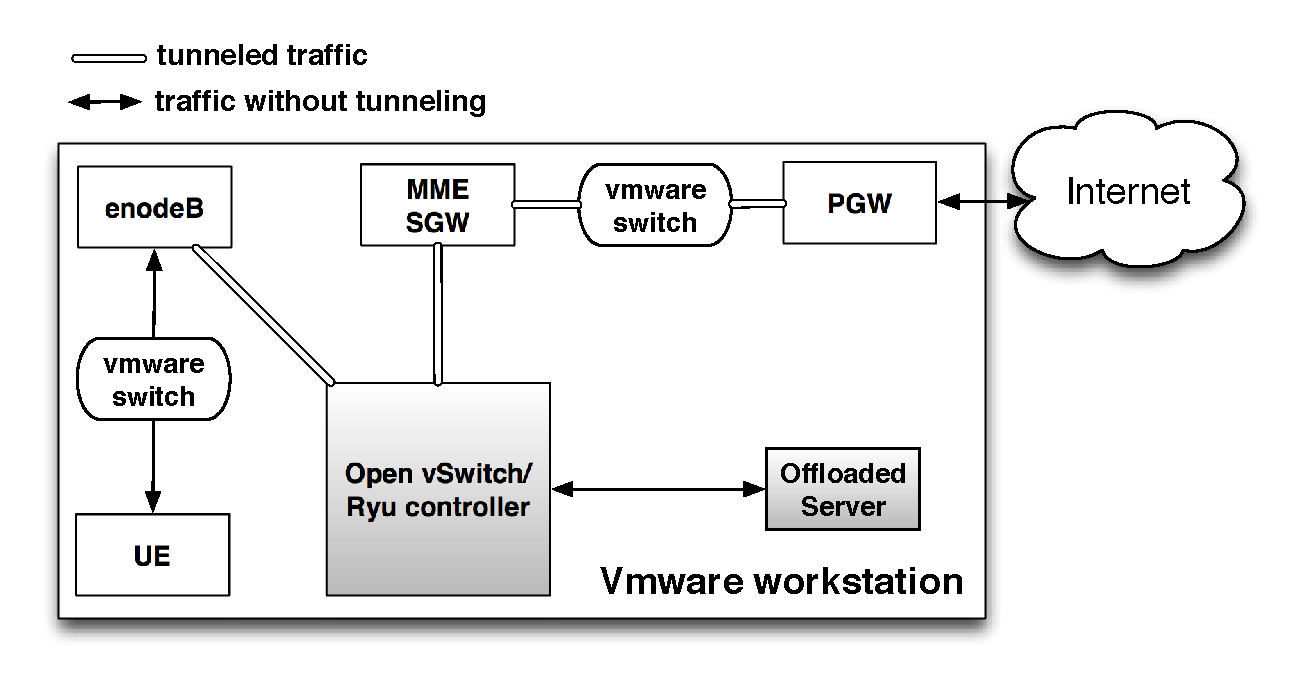
\epsfig{file=./figure/testbed, width=8cm} %height=5.5cm , 
\caption{Openepc testbed}
\label{fig:testbed}
\end{figure}

We used openepc testbed for mobile network. It includes all the components and a major part of the functionality of the EPC as well as supports a variety of radio access network (e.g. 2G, 3G, LTE, WiFi, and WiMax )  and UE by an emulation. We deployed the openepc testbed in Emulab with vmware workstation and Figure~\ref{fig:testbed} shows the deployed system. 
Each box is one of the vm instance and two vms which are depicted as gray boxes are added for our prototype. The lines with an arrow mean the connection without GTP tunnel and the lines without arrow mean connection with GTP tunnel.


\subsection{Prototype Implementation}

To implement prototype, we used Open vSwitch(OVS) version 2.0 and Ryu controller which support OpenFlow 1.3 standard. The OVS has the three ports which are connected to enodeB, MME\&SGW, and Offloaded Server shown in Figure~\ref{fig:testbed}. 

When the controller first runs, it sets up three matching rules in OVS tables. 
First matching rule is for forwarding GTP-U packet to a controller to a controller by using \textit{OXM\_OF\_UDP\_DST} field because all of the GTP-U packets have the same UDP destination port number(2152).  Second matching rule is for forwarding the packets from a offloaded server by using \textit{OXM\_OF\_TCP\_SRC} filed. Whenever new offloaded servers are launched in core network(CN), the controller sets up the matching rules with their IP address. 
The last matching rules is to forward the rest of packets like control plane data which does not match first and second rules without contacting a controller. The rules is set up with \textit{OXM\_OF\_IN\_PORT} and should have lower priority than first and second rules. 

However, current OVS does not support GTP encapsulation and decapsulation  and OpenFlow standard does not define the GTP. So, we implemented the python library with \textit{struct}~\cite{py_struct}  module in ryu controller for the encapsulation and decapsulation of GTP-U packets in a controller. 

Whenever UE sends packets to a server, the first matching rule is matched and the packet is forwarded to a controller. The controller decapsulates the GTP-U packet and checks if the destination IP address is the same as the offloaded server or not. If so, it removes the MAC, IP, UDP, and GTP-U layers from a packet and then forwards it to a offloaded server. The controller keeps the mapping table which stores mac and IP address of enodeb and SGW for GTP-U encapsulation of returning packet with UE’s IP address as key. Otherwise, the packet without a decapsulation is sent to the port which is connected to SGW. 

When the offloaded server sends the packet to UE, the second rule is matched and the packet is forwarded to a controller. The controller checks the mapping tables with destination ip address from a packet and encapsulates it with stored data. Then, it sends the encapsulated packet to port which is connected to enodeb.
